\documentclass[aspectratio=169]{beamer}

\usetheme{Rochester}
\usecolortheme{default}
\usepackage{amsmath, amssymb}
\usepackage{graphicx}
\usepackage{booktabs}

% --- convenience ---
\newcommand{\mpl}{M_{\mathrm{Pl}}}

\title[PBHs from resonance during inflation]{The formation of primordial black holes due to resonant processes during cosmic inflation}
\author{Gytis Vejelis}
\institute{Vilnius University, Faculty of Physics\\Theoretical Physics and Astronomy Institute}
\date{2026}

\begin{document}

% =========================================================
\begin{frame}
  \titlepage
\end{frame}

% --------------------- INTRO (about 60%) ------------------
\begin{frame}{Motivation \& big picture}
\begin{itemize}
  \item Inflation: early accelerated expansion; solves horizon/flatness problems via quasi-exponential growth.
  \item Quantum fluctuations $\rightarrow$ curvature/density perturbations $\rightarrow$ structure formation.
  \item Rare large perturbations on small scales can collapse after horizon re-entry $\rightarrow$ primordial black holes (PBHs).
  \item Goal of this project: build numerical tools + study inflaton dynamics (first in a simplified limit), as a step toward resonance-driven enhancement relevant for PBHs.
\end{itemize}
\end{frame}

\begin{frame}
  \begin{center}
    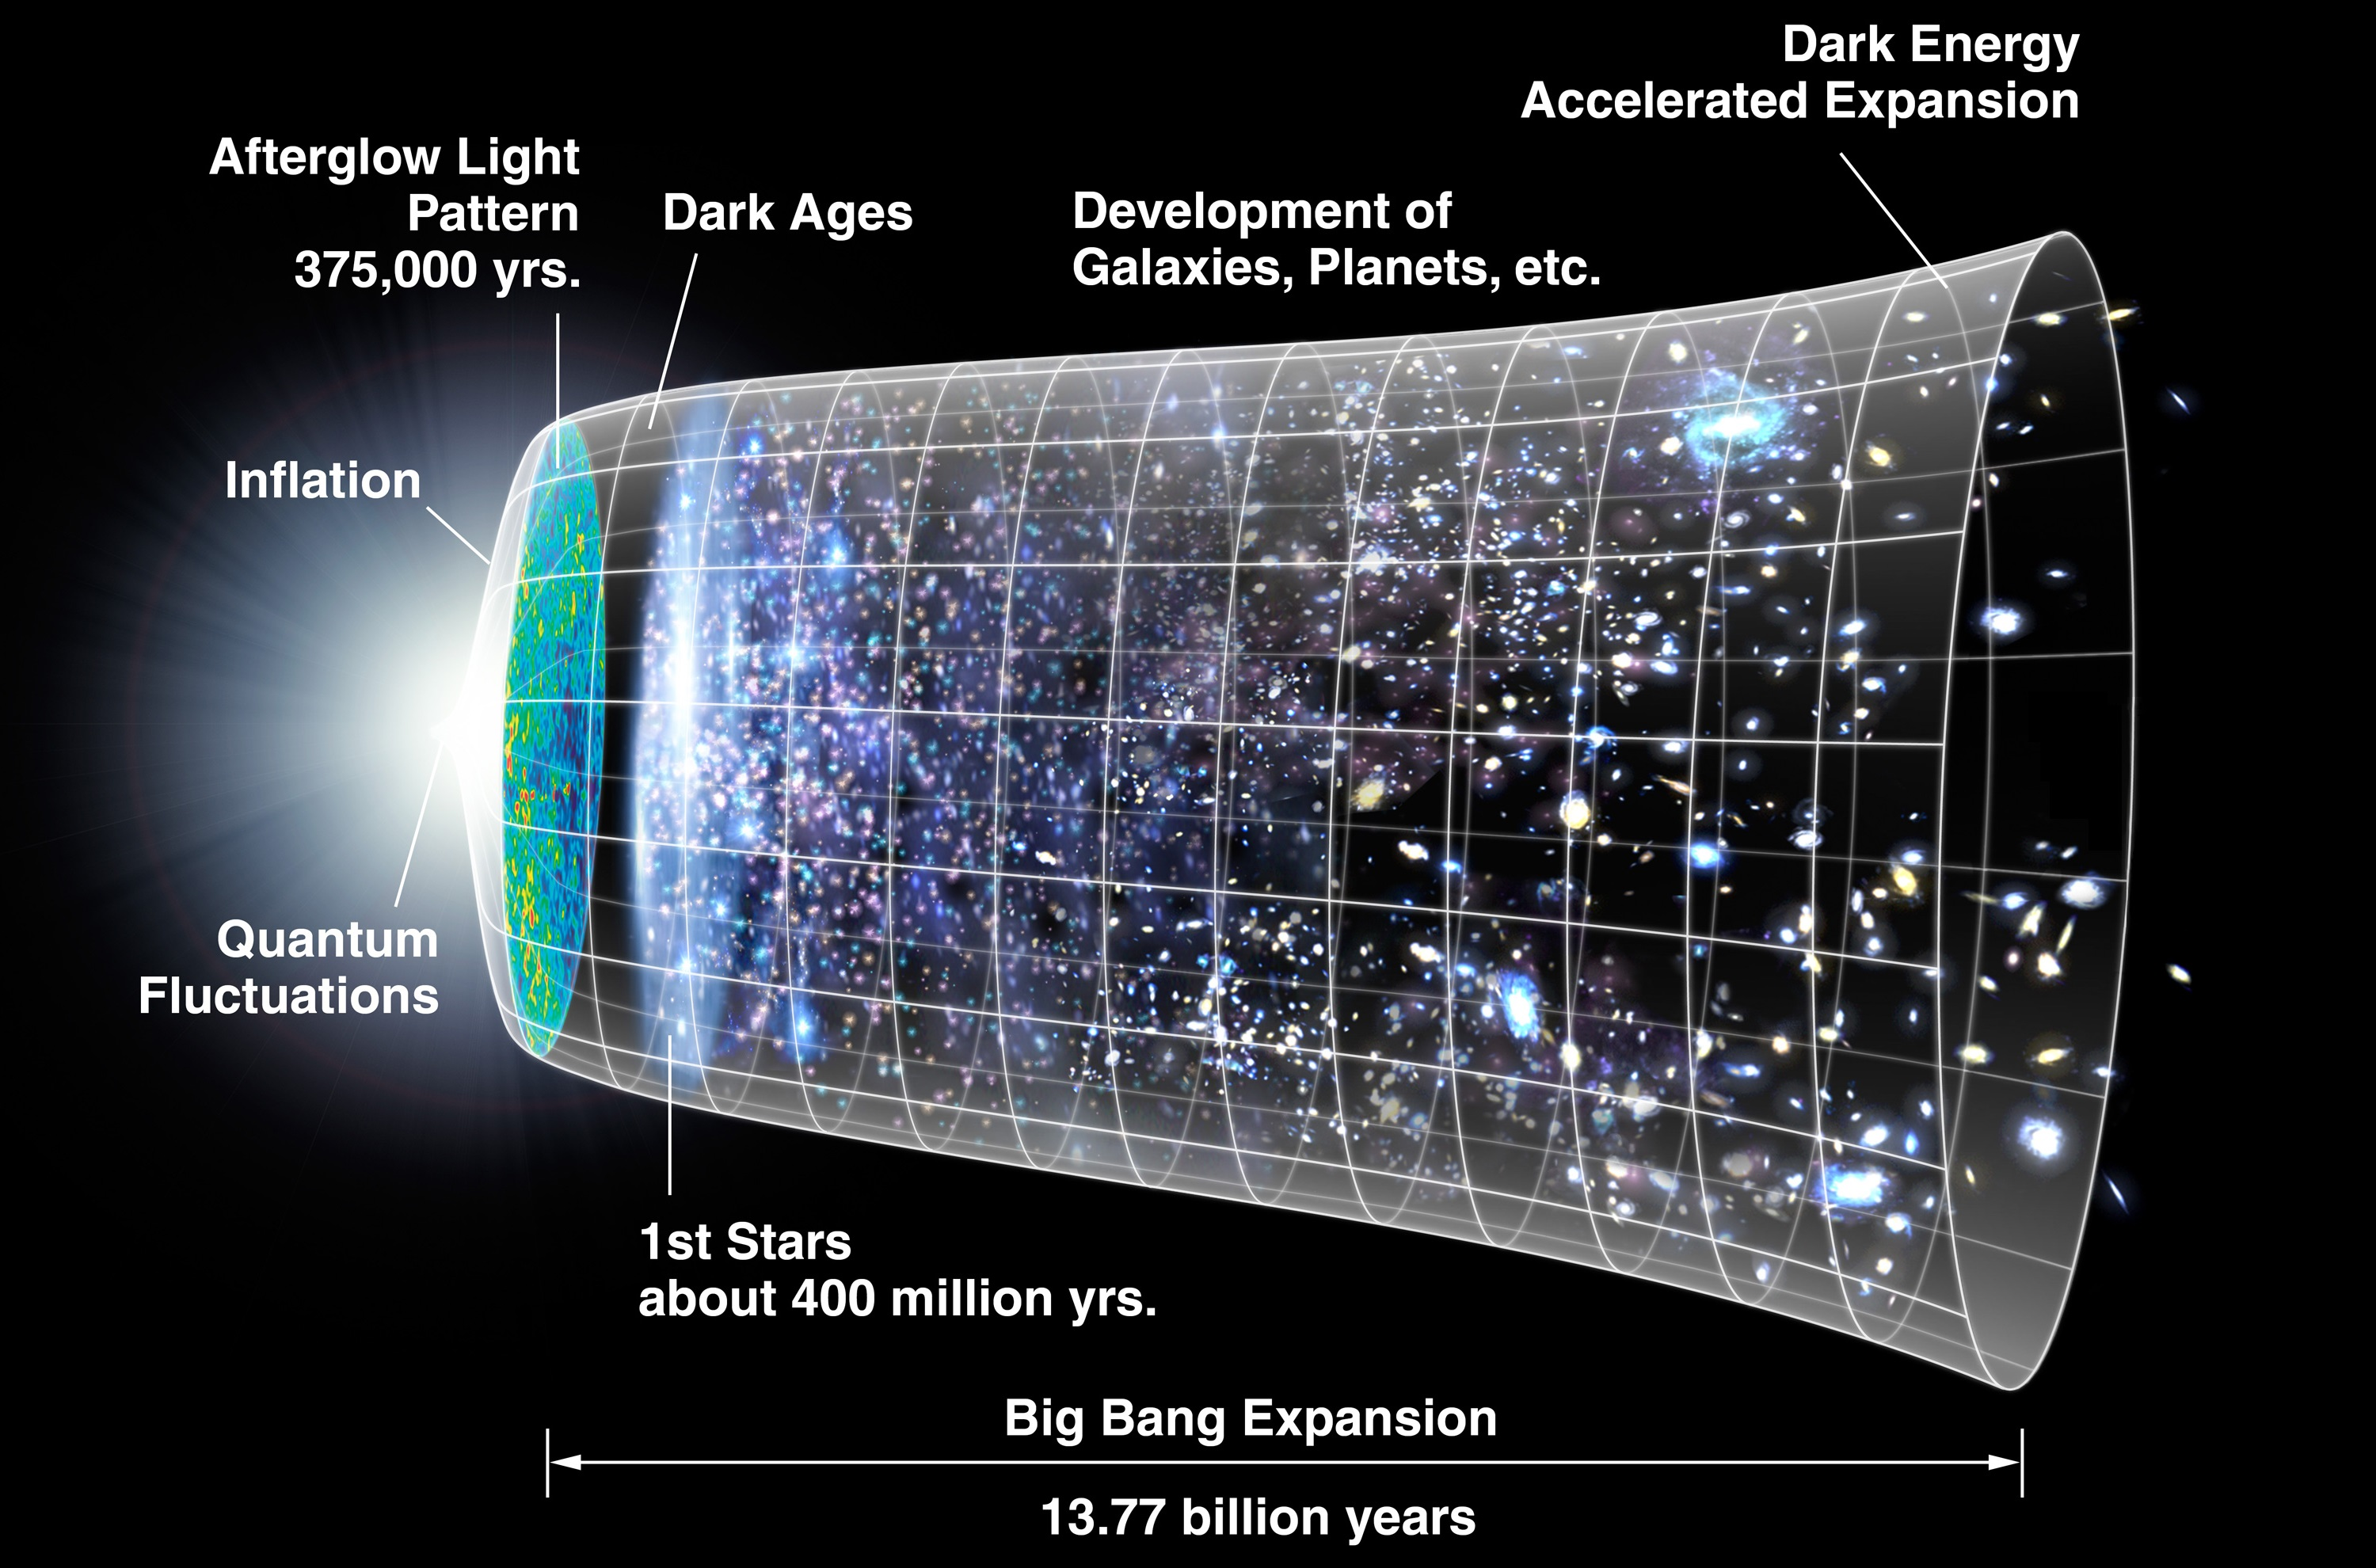
\includegraphics[width=300pt]{images/cmb_timeline.jpg}
  \end{center}
  \vspace{2mm}
    {\footnotesize Source: Wikipedia: Big Bang}
\end{frame}

\begin{frame}{Background: FLRW + inflation conditions}
Assume homogeneity/isotropy $\Rightarrow$ FLRW metric and perfect-fluid stress tensor.
\begin{itemize}
  \item Friedmann equations:
  \[
    H^2=\left(\frac{\dot a}{a}\right)^2=\frac{8\pi G}{3}\rho-\frac{k}{a^2},\qquad
    \frac{\ddot a}{a}=-\frac{4\pi G}{3}(\rho+3p).
  \]
  \item Accelerated expansion requires $\ddot a>0 \iff \rho+3p<0$.
  \item Model inflation with a scalar inflaton $\phi$ and potential $V(\phi)$.
\end{itemize}
\end{frame}

\begin{frame}{Inflaton dynamics and slow-roll parameters}
Scalar-field equation in an expanding background:
\[
  \ddot\phi+3H\dot\phi+V_{,\phi}=0.
\]
Useful parameters:
\[
  \epsilon \equiv -\frac{\dot H}{H^2},\qquad
  \epsilon=\frac{\dot\phi^{\,2}}{2\mpl^2 H^2},\qquad
  \eta \equiv \frac{\dot\epsilon}{H\epsilon}.
\]
\begin{itemize}
  \item Inflation: $\epsilon<1$; end of inflation: $\epsilon=1$.
  \item Slow-roll: $\dot\phi^2 \ll V(\phi)$ and $\epsilon,\eta\ll 1$.
  \item Kination (opposite regime): kinetic energy dominates, $\rho_\phi\propto a^{-6}$.
\end{itemize}
\end{frame}

\begin{frame}{Reheating vs preheating}
After inflation, the inflaton must transfer energy to matter degrees of freedom.
\begin{itemize}
  \item \textbf{Reheating (perturbative)}: inflaton decays with rate $\Gamma$; radiation bath forms, rough end when $H\sim \Gamma$.
  \item \textbf{Preheating (non-perturbative)}: early stage with resonant instabilities and rapid particle production.
  \item A typical example: coupling to a scalar $\chi$ gives time-dependent effective frequency $\omega_k(t)$ for modes $\chi_k$.
\end{itemize}
\end{frame}

\begin{frame}{Parametric resonance and Mathieu equation}
In a simplified preheating setup (neglect expansion over short times), mode equation becomes Mathieu:
\[
  \chi_k'' + \left(A_k - 2q\cos 2z\right)\chi_k=0,
\qquad
A_k=\frac{k^2}{m^2}+2q,\quad
q=\frac{g^2\Phi^2}{4m^2}.
\]
\begin{itemize}
  \item Floquet theory $\Rightarrow$ instability bands where $\chi_k$ grows exponentially.
  \item Particle production tracked via comoving occupation number $n_k$ (computed from mode functions and $\omega_k$).
\end{itemize}
% --- Insert Fig. 1 from your paper (page ~10) ---
% \includegraphics[width=0.80\linewidth]{fig1_mathieu_stability.png}
\end{frame}

\begin{frame}{Stability curves}
    \begin{center}
        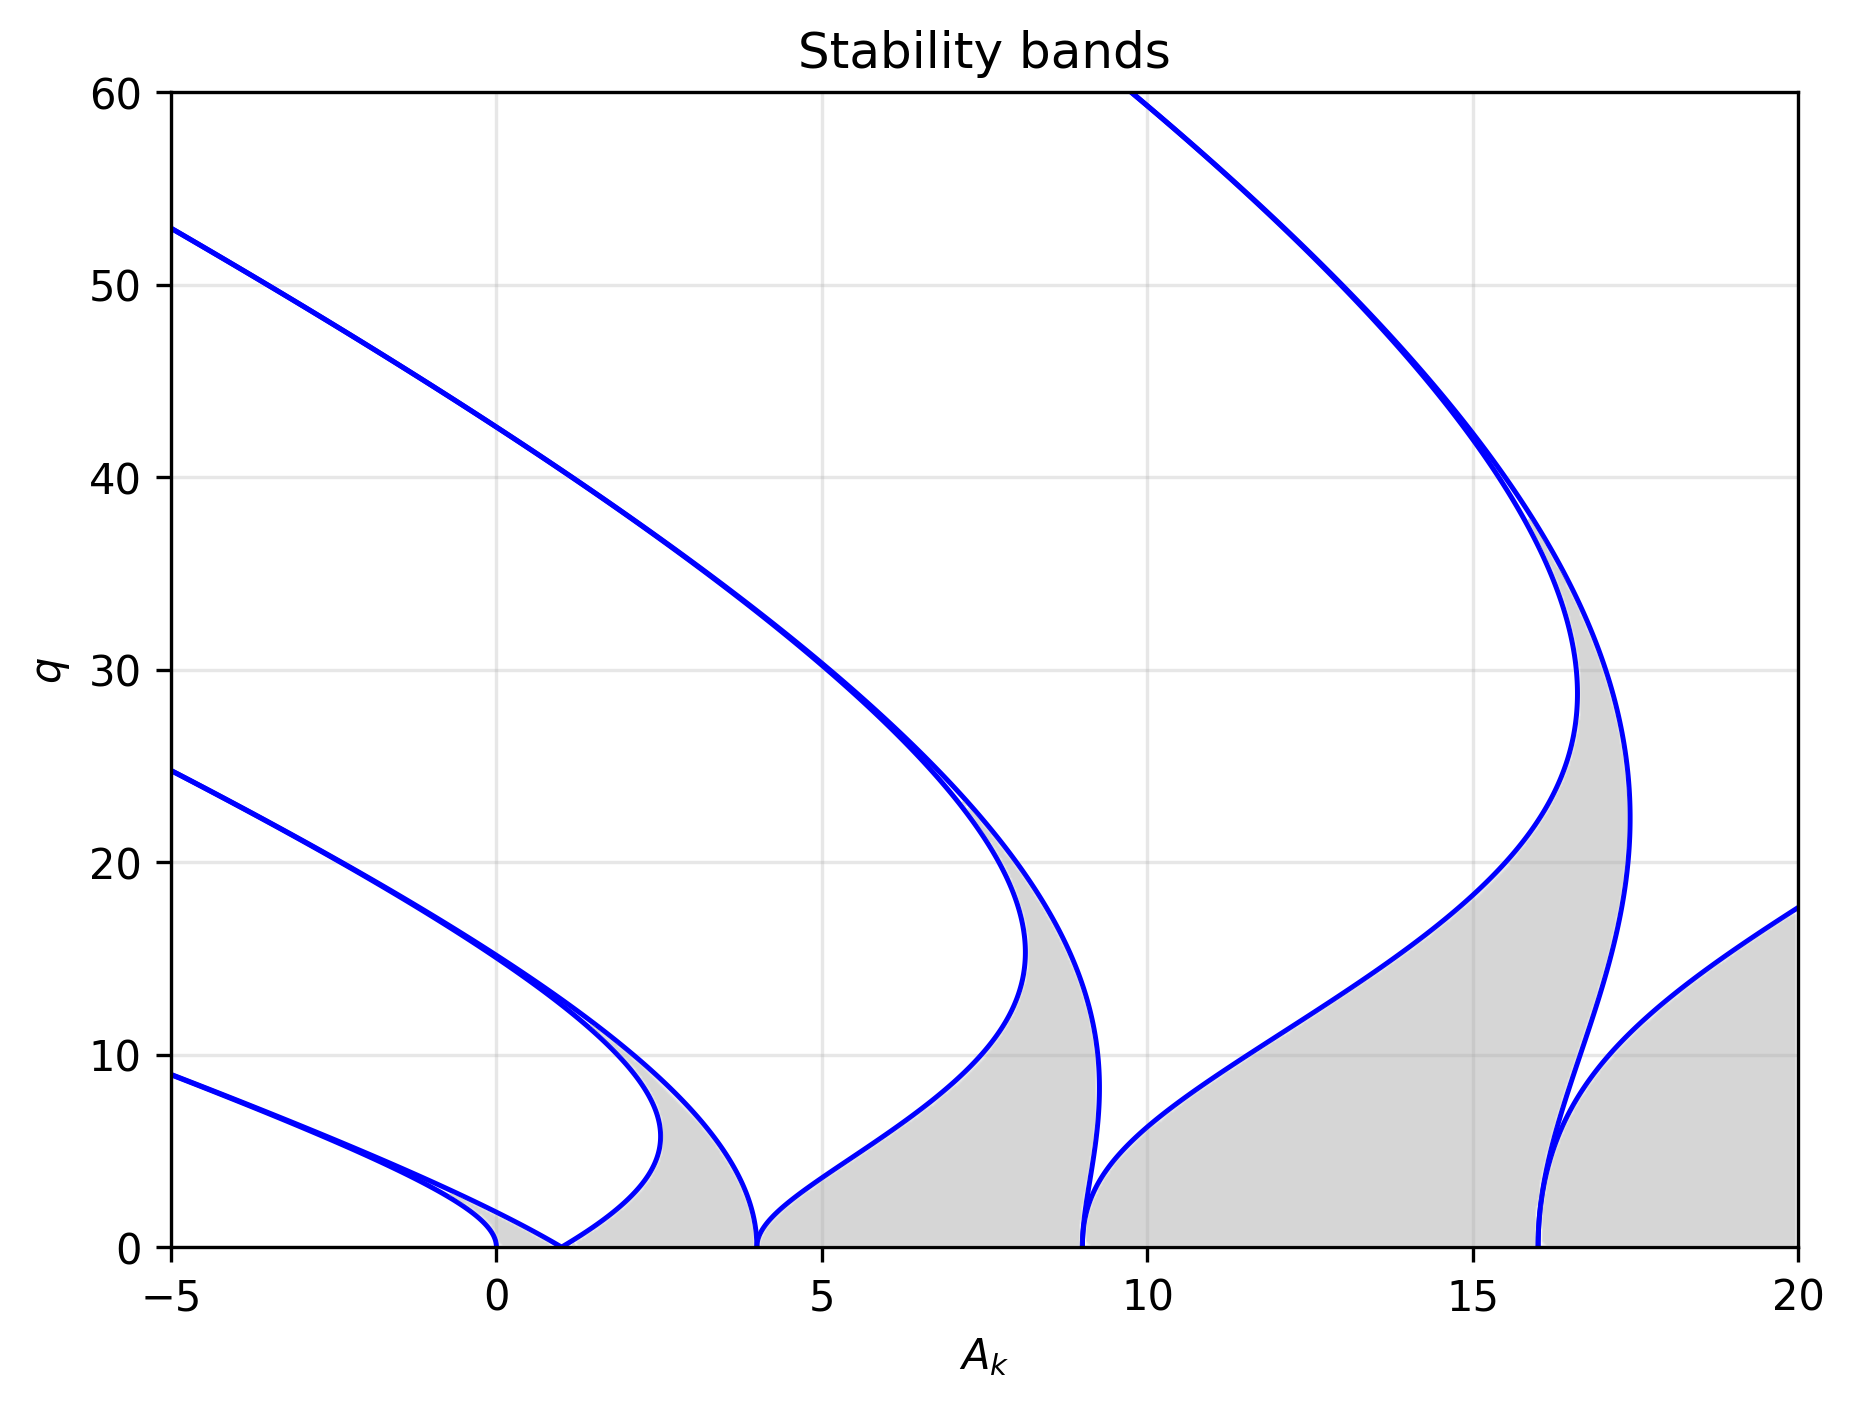
\includegraphics[width=250pt]{images/matheius_curves.png}
    \end{center}
\end{frame}

\begin{frame}{PBHs from metric perturbations: Newtonian gauge picture}
Perturbed FLRW in Newtonian gauge:
\[
  ds^2=-(1+2\Phi)\,dt^2 + a(t)^2(1-2\Phi)\delta_{ij}dx^i dx^j.
\]
\begin{itemize}
  \item Field perturbations $\delta\phi_k,\delta\chi_k$ couple to metric perturbation $\Phi_k$.
  \item From solutions one constructs curvature perturbation $\zeta_k$ and its power spectrum:
  \begin{equation*}
    P_\zeta(k)=\frac{k^3}{2\pi^2}\,|\zeta_k|^2 \quad \text{with} \quad \zeta_k
= \Phi_k + 2H\,\frac{\dot{\Phi}_k + H\Phi_k\left(1+\frac{1}{3}\frac{k^2}{a^2H^2}\right)}
{\dot{\phi}^2 + \dot{\chi}^2}. 
  \end{equation*}
  \item PBH idea: if small-scale $P_\zeta(k)$ is enhanced, overdense regions can collapse upon horizon re-entry (radiation era).
\end{itemize}
\end{frame}

\begin{frame}{Numerics: RK4 strategy}
We solve ODE systems by rewriting second-order equations into first-order vector form:
\begin{equation*}
  x'' = F(x,x',t)\quad \Rightarrow\quad
  \begin{cases}
    x' = v,\\
    v' = F(x,v,t).
  \end{cases}
\end{equation*}
RK4 update (conceptually): use four slope evaluations per step and a weighted average to advance the state.
\begin{itemize}
  \item Initialize $\dot\phi_0$ from slow-roll estimate.
  \item Integrate until end of inflation determined by $\epsilon=1$.
  \item Record $N_{\mathrm{end}}$ and diagnostics (e.g., particle-production indicator).
\end{itemize}
\end{frame}

% --------------------- RESULTS (about 40%) ----------------
\begin{frame}{Model used in Results: potential + extended field content}
Lagrangian includes inflaton $\phi$ and complex scalar $\psi$ with self-interaction:
\begin{equation*}
\mathcal{L} = \frac{1}{2}\nabla_\mu\phi\nabla^\mu\phi
+ \nabla_\mu\psi^*\nabla^\mu\psi
- V(\phi) - \frac{1}{2}m_\psi^2(\phi)|\psi|^2 - \frac{\lambda}{4}|\psi|^4 - \frac{\lambda}{4}f^4,
\end{equation*}
with
\begin{equation*}
m_\psi^2(\phi)=g^2(\phi-\phi_{\mathrm{SBP}})^2-\lambda f^2.
\end{equation*}
Inflationary potential studied (exponential-to-exponential form):
\begin{equation*}
V(\phi)=V_0\exp\!\left[-\kappa \exp\!\left(\frac{\phi}{b\mpl}\right)\right].
\end{equation*}
\end{frame}

\begin{frame}{Shape of the potential}
    \begin{center}
        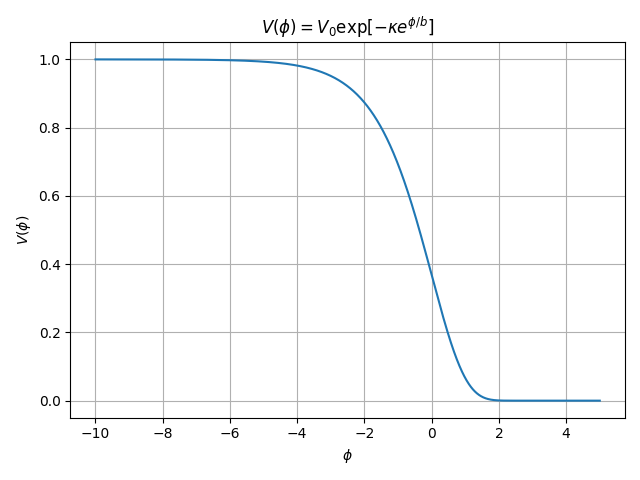
\includegraphics[width=250pt]{images/potential.png}
    \end{center}
\end{frame}

\begin{frame}{Illustration of the potential}
    \begin{center}
        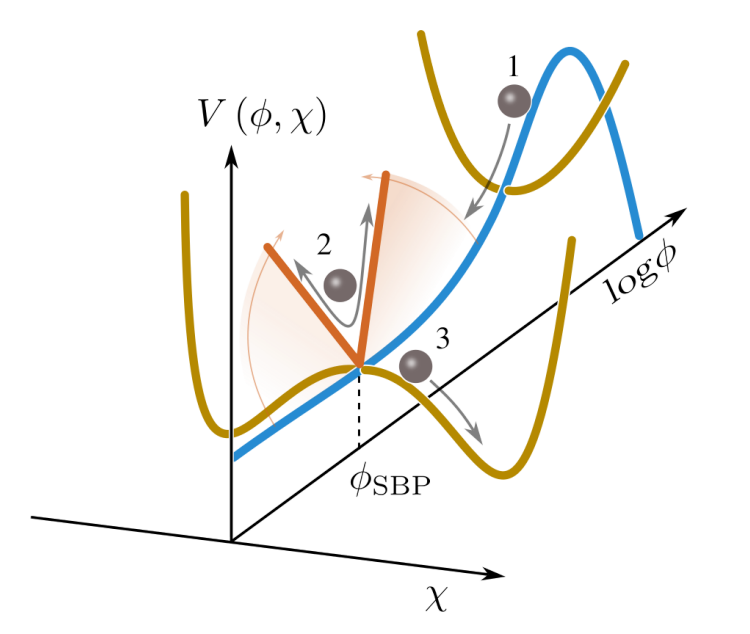
\includegraphics[width=220pt]{images/potential illustration.png}
    \end{center}
    \vspace{2mm}
    {\footnotesize Source: Y. S. Furuta, et al., Primordial Black Holes as Dark Matter and the Tachyonic Trap During Inflation, 11 2025.}
\end{frame}

\begin{frame}{Derived equations}
    \begin{equation*}
    \ddot{\phi} + 3H \dot{\phi}
    - \frac{\kappa V_0}{b M_{\rm Pl}}
    \exp\!\left[\frac{\phi}{b M_{\rm Pl}} - \kappa e^{\frac{\phi}{b M_{\rm Pl}}}\right]
    + g^2 \langle \chi^2 \rangle (\phi - \phi_{\rm SBP}) = 0
    \end{equation*}

    \begin{equation*}
    \ddot{\tilde{\chi}}_{\mathbf{k}} + 3H \dot{\tilde{\chi}}_{\mathbf{k}}
    + \left[
    \frac{k^2}{a^2}
    + g^2 (\phi - \phi_{\rm SBP})^2
    - \lambda f^2
    + 3 \lambda \langle \chi^2 \rangle + \langle \dot{\theta}^2 \rangle
    + \frac{1}{a^2} \langle (\nabla \theta)^2 \rangle
    \right]
    \tilde{\chi}_{\mathbf{k}} = 0
    \end{equation*}

    \begin{equation*}
    \langle \chi^2 \rangle \ddot{\tilde{\theta}}_{\mathbf{k}}
    + (2 \langle \chi \dot{\chi} \rangle + 3H \langle \chi^2 \rangle) \dot{\tilde{\theta}}_{\mathbf{k}}
    + \frac{k^2}{a^2} \langle \chi^2 \rangle \tilde{\theta}_{\mathbf{k}} = 0
    \end{equation*}
    where the averages are

    \begin{equation*}
    \langle \chi^2 \rangle
    = \int_{\mathbb{R}^3} \frac{d^3 p}{(2\pi)^3}
    \left[ |\tilde{\chi}_{\mathbf{p}}(t)|^2 + \text{2PI-corrections} \right]
    \end{equation*}

    \begin{equation*}
    \langle \dot{\theta}^2 \rangle
    = \int_{\mathbb{R}^3} \frac{d^3 p}{(2\pi)^3}
    \left[ |\dot{\tilde{\theta}}_{\mathbf{p}}(t)|^2 + \text{2PI-corrections} \right]
    \end{equation*}
\end{frame}

\begin{frame}{Analytic checks (slow-roll and kination limits)}
Slow-roll in $N=\ln a$ gives a closed-form reference solution (used to validate numerics):
\[
\phi(N)= -b \ln\!\left(\frac{\kappa}{b^2}(N_0-N)\right).
\]
Kination attractor (kinetic dominated):
\[
\phi(N)=\phi_* \pm \sqrt{6\,(N-N_*)}.
\]
\begin{itemize}
  \item These limits provide sanity checks: numerical $\phi(N)$ should match slow-roll early, and approach kination-like behavior when appropriate.
\end{itemize}
\end{frame}

\begin{frame}{Numerical inflaton evolution and end of inflation}
In the simplified \textbf{inflaton-only} approximation ($\langle\chi\rangle=\langle\theta\rangle=0$), RK4 integration yields:
\begin{itemize}
  \item Rapid growth of $\phi(N)$ in the chosen potential.
  \item End of inflation at approximately:
  \[
    N_{\mathrm{end}} \approx 12.59 \quad (\epsilon=1).
  \]
  \item Post-inflation dynamics are unrealistic without energy transfer/backreaction (only Hubble friction present).
\end{itemize}
\end{frame}

\begin{frame}
    \begin{center}
        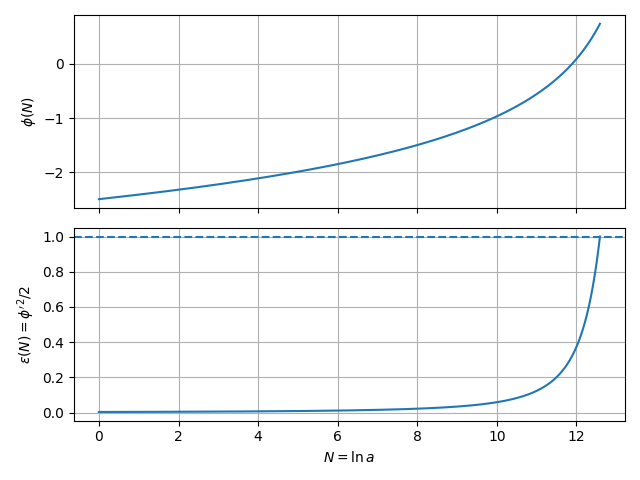
\includegraphics[width=250pt]{images/phi evolution.png}
    \end{center}
\end{frame}

\begin{frame}{Particle-production indicator and interpretation}
Comoving occupation-number indicator shows step-like growth:
\begin{itemize}
  \item In comoving variables, $\ln n_k$ can exhibit jumps and temporary drops (coordinate/definition artifact).
  \item In a more complete treatment (including coupled $\chi,\theta$ + backreaction), effective friction and energy transfer should modify both $\phi(N)$ and particle production.
\end{itemize}
\end{frame}

\begin{frame}
    \begin{center}
        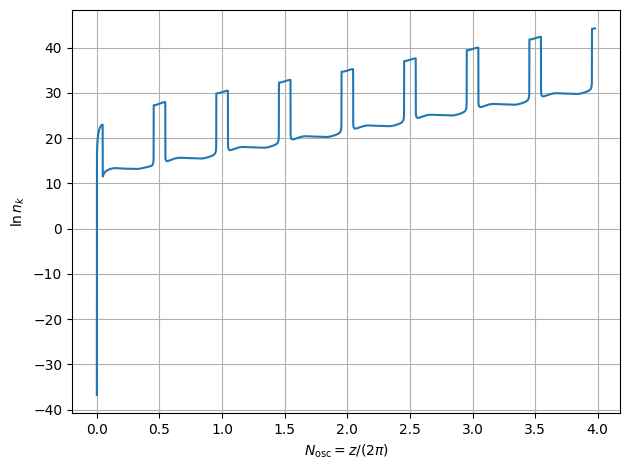
\includegraphics[width=250pt]{images/particle production phi.png}
    \end{center}
\end{frame}

\begin{frame}{Takeaways \& next steps toward PBHs}
\begin{itemize}
  \item Built RK4-based framework and validated inflaton evolution against analytic limits.
  \item Found $N_{\mathrm{end}}\approx 12.59$ for the inflaton-only evolution in this potential.
  \item Next steps:
    \begin{itemize}
      \item Couple in $\chi,\theta$ dynamics and compute averages $\langle\chi^2\rangle$,
      \item Track resonance-driven amplification and propagate into metric perturbations $\Phi_k$ and $P_\zeta(k)$.
      \item Identify parameter regions where small-scale $P_\zeta(k)$ is enhanced enough to support PBH formation.
    \end{itemize}
\end{itemize}
\end{frame}

% Optional: references slide (keep short for 10 min)
\begin{frame}{Key references}
\small
\begin{thebibliography}{9}
\bibitem{KLS1997} L. Kofman, A. Linde, A. A. Starobinsky, \emph{Phys. Rev. D} 56 (1997).
\bibitem{Furuta2025} Y. S. Furuta et al., \emph{Primordial Black Holes as Dark Matter and the Tachyonic Trap During Inflation} (2025).
\end{thebibliography}
\end{frame}

\end{document}
